\documentclass[../main.tex]{subfiles}
\begin{document}
\chapter{Results}
\label{hh:chapter:results}

This chapter presents the results obtained in the CMS HH~$\to$bb$\tau\tau$ analysis using the full Run 2 data set. Two sets of results: inclusive results, considering as signal both ggF and VBF altogether, and VBF-only results, where only the VBF production mode is considered as signal. 

This chapter is structured as follows. Section~\ref{hh:sec:stat} shows an overview of the statistical methodology followed for performing the signal extraction. Section~\ref{hh:sec:systematics} describes the systematic uncertainties considered in the analysis. The final results are shown in Section~\ref{hh:sec:results} and a comparison with the results obtained from other HH analyses is performed in Section~\ref{hh:sec:comparison}.

\section{Statistical procedure}
\label{hh:sec:stat}

The statistical methodology used to evaluate the presence or not of signals in data follows the method used in the 2011 combination of the CMS and ATLAS Higgs boson observation results \cite{hh:results:statistical_model}. This procedure, based on the modified frequentist method (often referred to as CL${}_\text{s}$), aims to quantify the compatibility between the observed data and the background plus signal hypothesis or between the data and the background only hypothesis. 

The procedure considers the DNN distributions in the categories (Resolved, 1 b-tag, Resolved 2 b-tag, Boosted and 5 VBF subcategories), three channels and three years (from here onwards, event categories) described during the analysis, for both the data, background estimate and signal processes. For each event category, the number of events $n_i$ predicted by the modelling in the bin $i$ of the distribution is defined as
\begin{equation}
n_i(\mu, \boldsymbol{\theta_i})=\mu\cdot s_i (\boldsymbol{\theta_i}) + b_i(\boldsymbol{\theta_i}),
\end{equation}
where $s_i (\boldsymbol{\theta_i})$ and $b_i(\boldsymbol{\theta_i})$ are the modelled signal and background yields in the given bin, $\mu$ is the \textit{signal strength modifier}, defined as the ratio between the observed signal cross section and the one predicted by the SM, and $\boldsymbol{\theta_i}$ are the \textit{nuisance parameters}, which parametrize the different uncertainties. These nuisance parameters are described in Section~\ref{hh:subsec:nuisances}.

\subsection{Observed and expected limits}

In order to estimate the values of the $\mu$ and their associated uncertainties, a binned \textit{likelihood function} is used to quantify the compatibility between the observed data and the prediction for given values of the statistical parameters ($\mu$ and nuisance parameters). This function can be written as the product of the Poisson probabilities to observe $n_i^{obs}$ events in the bin $i$, scaled by the prior nuisance probability distribution (defined in Section~\ref{hh:subsec:nuisances}):
\begin{equation}
L(\mu, \boldsymbol{\theta} | \text{data}) = \prod_i \frac{\left(\mu\cdot s_i (\boldsymbol{\theta_i}) + b_i(\boldsymbol{\theta_i}) \right)^{n_i^\text{obs}}}{n_i^\text{obs}!}e^{(\mu\cdot s_i (\boldsymbol{\theta_i}) + b_i(\boldsymbol{\theta_i}))} \cdot \rho(\boldsymbol{\theta_i}|\boldsymbol{\tilde{\theta_i}})
\end{equation}

To compare the compatibility of the data with  with different signal plus background hypotheses against the background-only hypothesis a \textit{test statistic} $q_\mu$ can be defined as:
\begin{equation}
q_\mu = -2 \ln \frac{L(\mu, \boldsymbol{\hat{\theta}}_\mu | \text{data})}{L(\hat{\mu}, \boldsymbol{\hat{\theta}} | \text{data})},
\end{equation}
where $\hat{\mu}$ and $\boldsymbol{\hat{\theta}}$ are the parameters that maximise $L$, and $\boldsymbol{\hat{\theta}}_\mu$ the set of nuisances that corresponds to the maximum value of $L$ for a given $\mu$ value. Higher values of $q_\mu$ correspond to increasing incompatibility of the data with the signal plus background hypothesis.

The probability density functions $f(q_\mu|\mu,\boldsymbol{\hat{\theta}}_\mu^\text{obs})$ (signal plus background hypothesis) and $f(q_0|0,\boldsymbol{\hat{\theta}}_0^\text{obs})$ (background-only) are obtained by generating pseudo-data, i.e. simulations that follow the same Poisson probability distribution. However, this approach is very CPU consuming, so instead an asymptotic approximation is considered \cite{hh:results:asymptotic}. Instead of using the generated pseudo-data, only the Asimov dataset (where the observations are equal to the predictions and the nuisance parameters are equal to their nominal values) is considered. Thus, the probabilities that the observed value $q_\mu^{n^{\text{obs}}}$ is compatible with the signal plus background ($\equiv$~CL$_{s+b}(\mu)$) or with the background-only ($\equiv$~CL$_{b}$) hypothesis are computed as
\begin{equation}
\begin{matrix}
\text{CL}_{s+b}(\mu) = P(q_\mu \geq q_\mu^{n^{\text{obs}}} | \mu\cdot s + b) = \int_{q_\mu^{n^{\text{obs}}}}^\infty f(q_\mu|\mu, \boldsymbol{\hat{\theta}}_\mu^\text{obs})~\text{d}q_\mu, \\
\text{CL}_{b} = P(q_0 \geq q_0^{n^{\text{obs}}} | b) = \int_{q_0^{n^{\text{obs}}}}^\infty f(q_0|\mu, \boldsymbol{\hat{\theta}}_0^\text{obs})~\text{d}q_0.
\end{matrix}
\end{equation}

Their ratio is known as the $\text{CL}_{s}(\mu)$,
\begin{equation}
\text{CL}_{s}(\mu) = \text{CL}_{s+b}(\mu) / \text{CL}_{b}.
\end{equation}

In the HH~$\to$~bb$\tau\tau$ analysis, the confidence level (CL) is taken as the value 1 - $\text{CL}_{s}$. The 95\% CL value ($\text{CL}_{s+b}(\mu) = 0.05$) is usually chosen as a convention for presenting CMS results.

The observed upper exclusion limit for the signal strength modifier $\mu_{\text{up}}$ is obtained so that $\text{CL}_{s}(\mu_{\text{up}})$ = 0.05. This observed limit can be compared with the expected exclusion limit (i.e. obtained only using the Asimov dataset) and its $\pm1\sigma$ or $\pm2\sigma$ error bands (corresponding to 68\% and 95\% confidence intervals respectively), so the agreement between the observations and the model predictions can be studied. In the asymptotic approach used, the N$\sigma$ error bands $\mu_{\text{up+N}}^\text{exp}$ and the median $\mu_{\text{up}}^\text{exp}$ of the expected limit are obtained using the Asimov dataset and given by \cite{hh:results:asymptotic}
\begin{equation}
\mu_{\text{up+N}}^\text{exp} = \sigma_A\cdot\left(\Phi^{-1}(1 - \text{CL}_s\Phi(N)) + \text{N}  \right),
\end{equation}
where $\sigma^2_A=\mu^2/q_{\mu, A}$ is evaluated by using the Asimov Dataset and $\Phi(x)$ is the cumulative standard Gaussian distribution (zero mean, unit variance).


\subsection{Nuisance parameters}
\label{hh:subsec:nuisances}

Both background and signal event yields are affected by several sources of uncertainties, modelled by introducing nuisance parameters. These nuisance parameters have a probability density function $\rho(\theta|\tilde{\theta})$ associated to some estimate of the nominal value $\tilde{\theta}$ and other parameters regulating its shape. Due to the Bayes' theorem, the probability density can be re-interpreted as a posterior arising from dedicated measurements for the estimations of $\tilde{\theta}$:
\begin{equation}
\rho(\theta|\tilde{\theta}) \sim p(\theta|\tilde{\theta}) \cdot \pi_\theta(\theta),
\end{equation}
where $p(\theta|\tilde{\theta})$ is the probability density function for the auxiliary measurement of $\tilde{\theta}$ and $\pi_\theta(\theta)$ the prior probability distribution.

In the HH$\to$bb$\tau\tau$ analysis, three types or nuisances are considered. 
\begin{itemize}
\item Normalization uncertainties: some uncertainties only modify the normalization of one or more processes, affecting either all event categories or a limited number of those. Up and down variations of these uncertainties, obtained by adding or substracting to the bin content the value correspondent to one standard deviation to the central value, vary the number of events of the distribution equally in all bins. The prior probability distributions on these uncertainties involve Gaussian functions. However, for large values of the uncertainties, the normal distribution is not appropriate. Instead, the log-normal distribution is considered:
\begin{equation}
\pi_\theta(\theta) = \frac{1}{\theta}\frac{1}{\sqrt{2\pi}\sigma}\exp\left(-\frac{(\ln\theta)^2}{2\sigma^2}\right),
\end{equation}
where $\sigma$ is the width of the distribution and corresponds to the relative uncertainty on $\theta$, estimated using theoretical calculations or alternative measurements.

\item Shape uncertainties: instead of only modifying the whole integral of the distributions, some uncertainties vary the content of individual bins in an event category distribution. These variations are modelled by recreating the distributions by modifying the quantity affected by the systematic according to the boundaries of its central 68\% confidence interval. Using the three distributions (no variation and up and down variations), the number of events per bin is smoothly interpolated between the boundaries defined by the up and down distributions.

\item Statistical uncertainties: the amount of simulated events that can be produced for a given process per bin and event category is limited. To model the statistical uncertainties, one possibility is to include one separate nuisance per process and bin following a Poisson distribution, the so-called Barlow-Beeston approach  \cite{hh:results:barlow_beeston}. However, if enough events are available per bin, the sum of Poisson distributions can be approximated by a Gaussian distribution with reasonable accuracy. In that case, only one nuisance per bin is incorporated in the statistical model.
\end{itemize}

\subfile{systematics}



\section{Results}
\label{hh:sec:results}

The results shown in this section are obtained by performing a binned maximum likelihood fit of the DNN prediction in eight categories per channel simultaneously for all three years, resulting in a total of 72 input distributions. The three types of nuisance parameters introduced in Section~\ref{hh:subsec:nuisances} are considered, being the normalization and systematic uncertainties further described in Section~\ref{hh:sec:systematics}. 

The DNN output distributions for in 2018 for the $\tau_h\tau_h$ channel in the eight analysis categories is shown in Fig.~\ref{hh:fig:dnn_tautau}. The binning schemes used in the DNN distributions are chosen to minimise the expected upper limit, while keeping as low as possible the number of bins per distribution and ensuring the stability of the fit. Each bin is required to contain at least one t$\bar{\text{t}}$ and one Z$/\gamma^*$~+~jets event and to have a weighted background yield larger than 0.03.

%\begin{figure}
%\begin{center}
%\includegraphics[width=\textwidth]{Images/DNNplots_muTau_2018}
%\end{center}
%\caption{DNN prediction distributions in the \taumu\tauh{} channel in 2018 for the eight analysis categories. The shaded band in the plots represents the statistical plus systematic uncertainty. \textcolor{red}{Fuente de las figuras suplementarias?}}
%\label{hh:fig:dnn_mutau}
%\end{figure}
%
%\begin{figure}
%\begin{center}
%\includegraphics[width=\textwidth]{Images/DNNplots_eTau_2018}
%\end{center}
%\caption{DNN prediction distributions in the \taue\tauh{} channel in 2018 for the eight analysis categories. The shaded band in the plots represents the statistical plus systematic uncertainty. \textcolor{red}{Fuente de las figuras suplementarias?}}
%\label{hh:fig:dnn_etau}
%\end{figure}


\begin{figure}
\begin{center}
\includegraphics[width=\textwidth]{Images/DNNplots_tauTau_2018}
\end{center}
\caption{DNN prediction distributions in the \tauh\tauh{} channel in 2018 for the eight analysis categories. The shaded band in the plots represents the statistical plus systematic uncertainty. \textcolor{red}{Fuente de las figuras suplementarias?}}
\label{hh:fig:dnn_tautau}
\end{figure}



The expected and observed limits for the ggF + VBF HH production cross section at the SM and those for the VBF only HH production cross section are listed in Tables~\ref{hh:tab:limit_r} and \ref{hh:tab:limit_rvbf}, respectively. A visual representation of these limits is provided in Fig.~\ref{hh:fig:limits_r}.

\begin{table}[h!]
\begin{center}
\begin{tabular}{l | r | r}
& 
$
\begin{matrix}
\text{Obs. (Exp.) limit on } \\ \sigma_{\text{ggF+VBF}}(\text{pp}\to\text{HH})/ \sigma_{\text{ggF+VBF}}^{\text{theory}} 
\end{matrix}
$
& 
$
\begin{matrix}
\text{Obs. (Exp.) limit on } \\ \sigma_{\text{ggF+VBF}}(\text{pp}\to\text{HH}) \text{~[fb]}
\end{matrix}
$ \\ \hline
2016 &     8.9 (10.6) & 272 (324) \\
2017 &     9.5 (11.7) & 291 (356) \\
2018 &     5.5 (8.2)  & 169 (249) \\
Combined & 3.3 (5.2)  & 102 (159)
\end{tabular}
\end{center}
\caption{Expected and observed upper limits on the ratio of the experimentally expected  at 95\% CL for the SM point, where $\sigma_{\text{ggF+VBF}}^{\text{theory}}=32.776$~fb is the sum of the ggF and VBF HH production modes cross sections.}
\label{hh:tab:limit_r}
\end{table}


\begin{table}[h!]
\begin{center}
\begin{tabular}{l | r | r}
& 
$
\begin{matrix}
\text{Obs. (Exp.) limit on } \\ \sigma_{\text{VBF}}(\text{pp}\to\text{qqHH})/ \sigma_{\text{VBF}}^{\text{theory}} 
\end{matrix}
$
& 
$
\begin{matrix}
\text{Obs. (Exp.) limit on } \\ \sigma_{\text{VBF}}(\text{pp}\to\text{qqHH}) \text{~[fb]}
\end{matrix}
$ \\ \hline
2016 &     283 (357) & 487 (616) \\
2017 &     280 (392) & 485 (676) \\
2018 &     241 (226) & 414 (391) \\
Combined & 124 (154) & 212 (266)
\end{tabular}
\end{center}
\caption{Expected and observed upper limits on the ratio of the experimentally expected  at 95\% CL for the SM point, where $\sigma_{\text{VBF}}^{\text{theory}}=1.726$~fb is the VBF HH production mode cross section.}
\label{hh:tab:limit_rvbf}
\end{table}


\begin{figure}[h!]
\begin{center}
\subfloat{\includegraphics[width=0.5\textwidth]{Images/Figure_007-a}}
\subfloat{\includegraphics[width=0.5\textwidth]{Images/Figure_007-b}}
\end{center}
\caption{Expected and observed upper limits on the ratio of experimentally expected (left) ggF + VBF ($\sigma_{\text{ggF+VBF}}$) and (right) VBF only ($\sigma_{\text{VBF}}$) HH production cross section and the expectation from the SM ($\sigma_\text{theory}$) at 95\%, splitted by the different years and combined for the full Run 2 dataset. Extracted from \cite{hh:analysis:run2}.}
\label{hh:fig:limits_r}
\end{figure}

In order to study the Higgs couplings involved, the upper limits on the HH production cross section can also be computed for fixed values of the parameters. Fig.~\ref{hh:fig:limits_r} shows the scans of the expected and observed upper limits on the HH production cross sections as functions of $\kappa_\lambda$ (ggF + VBF) and \kvv{} (VBF only). With 95\% CL, $\kappa_\lambda$ gets constrained between $ -1.7 <\kappa_\lambda < 8.7$ (observed) and $-2.9 < \kappa_\lambda < 9.8$ (expected) and \kvv{} between $-0.4 <$~\kvv{}~$< 2.6$ (observed) and $-0.6<$~\kvv{}~$<  2.8$ (expected). In both cases, the other couplings are set to 1 (i.e. SM value).

\begin{figure}[h!]
\begin{center}
\subfloat{\includegraphics[width=0.5\textwidth]{Images/Figure_008-a}}
\subfloat{\includegraphics[width=0.5\textwidth]{Images/Figure_008-b}}
\end{center}
\caption{Expected and observed upper limits on the experimentally expected (left) ggF + VBF ($\sigma_{\text{ggF+VBF}}$) HH production cross section as functions of $\kappa_\lambda$ and (right) VBF only ($\sigma_{\text{VBF}}$) HH production cross section as functions of \kvv. In both cases, all the other couplings are set to their SM expectations. The red solid lines show the theoretical prediction for the HH production cross sections and its uncertainty (red shaded bands). Extracted from \cite{hh:analysis:run2}.}
\label{hh:fig:limits_r}
\end{figure}

%Fig.~\ref{hh:fig:limits_r} shows the two-dimensional scans of the expected and observed upper limits on the HH production cross sections as functions of $\kappa_\lambda$ and $\kappa_t$ (ggF + VBF) and \kvv{} and $\kappa_V$ (VBF only). A point in a two-dimensional parameter space is excluded when the upper limit on HH production cross section at 95\% CL is measured to be below the theoretical cross section, evaluated at the corresponding parameter values. In both diagrams, the SM point is included inside the constrained area.
%
%
%\begin{figure}[h!]
%\begin{center}
%\subfloat{\includegraphics[width=0.5\textwidth]{Images/Figure_009-a}}
%\subfloat{\includegraphics[width=0.5\textwidth]{Images/Figure_009-b}}
%\end{center}
%\caption{Two-dimensional exclusion regions for the full Run-2 combination as a function (left) of $\kappa_\lambda$ and $\kappa_t$ with \kvv and $\kappa_V$ set to unity and (right) of \kvv{} and $\kappa_V$, with both $\kappa_\lambda$ and $\kappa_t$ fixed to unity. Expected uncertainties on exclusion boundaries are inferred from uncertainty bands of the limit calculation, and are denoted by dark and light-grey areas. The blue area marks parameter combinations observed to be excluded. Theoretical cross section values are illustrated by thin, labeled contour lines with the SM prediction (i.e. all parameters set to unity) denoted by a red diamond. Extracted from \cite{hh:analysis:run2}.}
%\label{hh:fig:limits_r_2d}
%\end{figure}

For both the ggF and VBF results reported, the largest sensitivity comes from the \tauh\tauh{} channel, followed by the \taumu\tauh{} and the \taue\tauh{} channels. The Resolved, 2 b-tag category provides the largest sensitivity when constraining the $\kappa_\lambda$ value, while the VBF subcategory is the most dominant in the \kvv{} measurement.


\section{Comparison with other HH analyses}
\label{hh:sec:comparison}

In this section a comparison between the results shown above and the ones provided by other analyses is performed.

First, within CMS the most direct comparison is with the HH$\to$bb$\tau\tau$ analysis using 2016 data published in 2018 \cite{hh:analysis:2016}. In this analysis, the signal extraction was performed by fitting the $m_{T2}$ distribution \cite{hh:analysis:mt2} and BDT was used in order to identify and reject the t$\bar{\text{t}}$ background. The observed (expected) limit on the measured HH production cross section at the SM point times the bb$\tau\tau$ branching fraction was found to be 75.4(61.0)~fb, correspondent to 31.5(25.5) times the cross section predicted by the SM. These numbers can be directly compared with the upper limits obtained in latest analysis using only 2016 data, shown in Tab.~\ref{hh:tab:limit_r} (observed (expected) limit of 8.9(11.0) times the SM prediction). Therefore, in the full Run-2 analysis we can see an improvement of $\sim$70\% in the observed limit and $\sim$58\% in the expected limit. Regarding the $\kappa_\lambda$ measurement, the 2016 analysis obtained observed (expected) constraints of $-18(-14) < k_\lambda < 26(22)$, a much wider range than the one obtained in the full Run-2 analysis. These new results benefit from the improved trigger strategy and the adoption of new techniques not only at analysis level, with the new neural network approaches used for categorization and signal extraction, but in the identification and reconstruction algorithms developed within the CMS Collaboration.

Considering the full Run-2 dataset, the ATLAS Collaboration also performed a HH$\to$bb$\tau\tau$ search \cite{hh:analysis:atlas, hh:analysis:atlas_comb}. Similarly to the CMS analysis, the signal extraction is performed by fitting the output score of a multivariate approach. Assuming a $\sigma_{\text{ggF+VBF}}^{\text{theory}}=32.7$~fb, the observed (expected) upper limit on the HH production cross section obtained was 4.7(3.9) times $\sigma_{\text{ggF+VBF}}^{\text{theory}}$. The value of $\kappa_\lambda$ is constrained between $-2.5 < \kappa_\lambda < 9.3$ (observed) and $-1.9 < \kappa_\lambda < 9.1$ (expected). These results are a bit more stringent than the CMS ones.

With respect to the VBF HH production, the ATLAS analysis did not perform a dedicated analysis for this production mode, although some results on the production cross section and the \kvv{} constraints were provided in the combination of ATLAS HH results \cite{hh:analysis:atlas_comb}. The observed (expected) upper limit on the VBF HH production cross section was found to be 433(366)~fb, while \kvv{} is constrained between $-0.5<~$\kvv{}$~<2.7$ (observed and expected). The value of the upper limit is much larger with respect to the one obtained in the CMS analysis, while the \kvv{} constraints are quite similar.

Regarding other CMS HH searches with Run-2 data, a combination of the CMS HH results was published to celebrate the tenth anniversary of the Higgs boson discovery \cite{hh:analysis:nature}. This combination includes five final states, and the bb$\tau\tau$ analysis ranks among the first three with the highest sensitivity (see Fig.~\ref{hh:fig:lim_comb}). 


\begin{figure}
\begin{center}
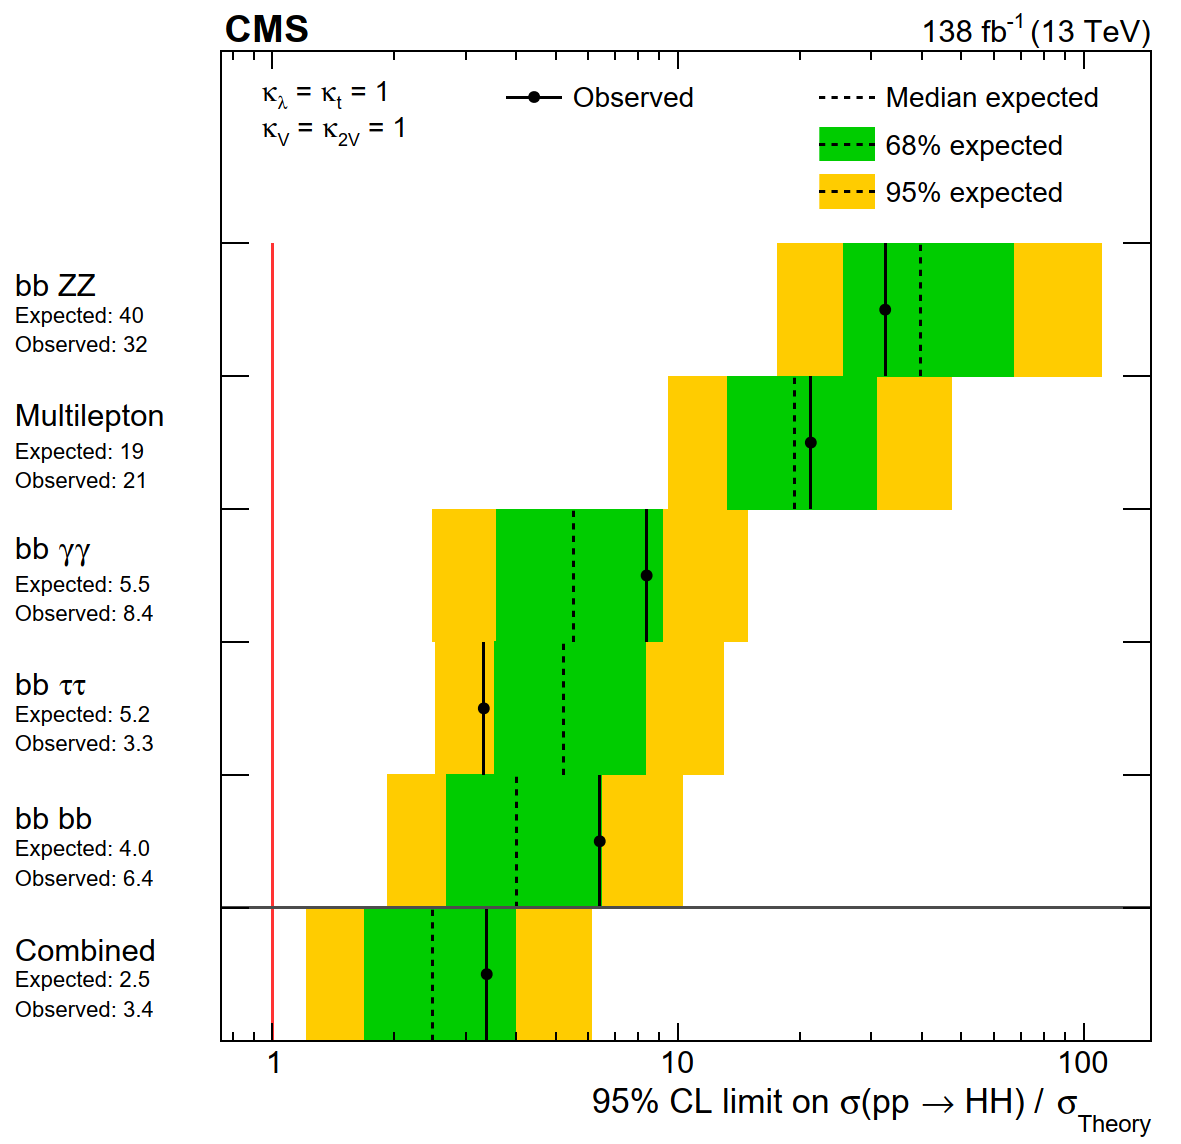
\includegraphics[width=0.7\textwidth]{Images/CMS-HIG-22-001_Figure_005-a}
\end{center}
\caption{Expected and observed limits on the ratio of experimentally estimated production cross section and the expectation from the SM $\sigma_{\text{Theory}}$ in searches using different final states and their combination. The search modes are ordered, from upper to lower, by their expected sensitivities from the least to the most sensitive. The overall combination of all searches is shown by the lowest entry. Extracted from \cite{hh:analysis:nature}.}
\label{hh:fig:lim_comb}
\end{figure}








\end{document}

